\documentclass{article}  
% Include all project wide packages here.
\usepackage{fullpage}
\usepackage{polyglossia}
\setmainlanguage{dutch}
\usepackage{csquotes}
\usepackage{graphicx}
\usepackage{epstopdf}
\usepackage{pdfpages}
\usepackage{caption}
\usepackage[list=true]{subcaption}
\usepackage{float}
%\usepackage{mathtools}
\usepackage{standalone}
\usepackage{import}
\usepackage{tocloft}
\usepackage{wrapfig}
\usepackage{authblk}
\usepackage{array}
\usepackage{booktabs}
\usepackage[toc,page,title,titletoc]{appendix}
\usepackage{xunicode}
\usepackage{amsmath}
\usepackage{fontspec}
\usepackage{unicode-math}
\usepackage[
    backend=bibtexu,
	texencoding=utf8,
bibencoding=utf8,
    style=ieee,
    sortlocale=nl_NL,
    language=auto
]{biblatex}
\usepackage{listings}
\newcommand{\includecode}[3][c]{\lstinputlisting[caption=#2, escapechar=, style=#1]{#3}}
\newcommand{\superscript}[1]{\ensuremath{^{\textrm{#1}}}}
\newcommand{\subscript}[1]{\ensuremath{_{\textrm{#1}}}}


\newcommand{\chapternumber}{\thechapter}
\renewcommand{\appendixname}{Bijlage}
\renewcommand{\appendixtocname}{Bijlagen}
\renewcommand{\appendixpagename}{Bijlagen}

\usepackage[hidelinks]{hyperref} %<--------ALTIJD ALS LAATSTE
  
\renewcommand{\familydefault}{\sfdefault}

\setmainfont[Ligatures=TeX]{Myriad Pro}
\setmathfont{Asana Math}
\setmonofont{Lucida Console}

\usepackage{titlesec, blindtext, color}
\definecolor{gray75}{gray}{0.75}
\newcommand{\hsp}{\hspace{20pt}}
\titleformat{\chapter}[hang]{\Huge\bfseries}{\chapternumber\hsp\textcolor{gray75}{|}\hsp}{0pt}{\Huge\bfseries}
\renewcommand{\familydefault}{\sfdefault}
\renewcommand{\arraystretch}{1.2}
\setlength\parindent{0pt}

%For code listings
\definecolor{black}{rgb}{0,0,0}
\definecolor{browntags}{rgb}{0.65,0.1,0.1}
\definecolor{bluestrings}{rgb}{0,0,1}
\definecolor{graycomments}{rgb}{0.4,0.4,0.4}
\definecolor{redkeywords}{rgb}{1,0,0}
\definecolor{bluekeywords}{rgb}{0.13,0.13,0.8}
\definecolor{greencomments}{rgb}{0,0.5,0}
\definecolor{redstrings}{rgb}{0.9,0,0}
\definecolor{purpleidentifiers}{rgb}{0.01,0,0.01}


\lstdefinestyle{csharp}{
language=[Sharp]C,
showspaces=false,
showtabs=false,
breaklines=true,
showstringspaces=false,
breakatwhitespace=true,
escapeinside={(*@}{@*)},
columns=fullflexible,
commentstyle=\color{greencomments},
keywordstyle=\color{bluekeywords}\bfseries,
stringstyle=\color{redstrings},
identifierstyle=\color{purpleidentifiers},
basicstyle=\ttfamily\small}

\lstdefinestyle{c}{
language=C,
showspaces=false,
showtabs=false,
breaklines=true,
showstringspaces=false,
breakatwhitespace=true,
escapeinside={(*@}{@*)},
columns=fullflexible,
commentstyle=\color{greencomments},
keywordstyle=\color{bluekeywords}\bfseries,
stringstyle=\color{bluestrings},
identifierstyle=\color{purpleidentifiers}
}

\lstdefinestyle{vhdl}{
language=VHDL,
showspaces=false,
showtabs=false,
breaklines=true,
showstringspaces=false,
breakatwhitespace=true,
escapeinside={(*@}{@*)},
columns=fullflexible,
commentstyle=\color{greencomments},
keywordstyle=\color{bluekeywords}\bfseries,
stringstyle=\color{redstrings},
identifierstyle=\color{purpleidentifiers}
}

\lstdefinestyle{xaml}{
language=XML,
showspaces=false,
showtabs=false,
breaklines=true,
showstringspaces=false,
breakatwhitespace=true,
escapeinside={(*@}{@*)},
columns=fullflexible,
commentstyle=\color{greencomments},
keywordstyle=\color{redkeywords},
stringstyle=\color{bluestrings},
tagstyle=\color{browntags},
morestring=[b]",
  morecomment=[s]{<?}{?>},
  morekeywords={xmlns,version,typex:AsyncRecords,x:Arguments,x:Boolean,x:Byte,x:Char,x:Class,x:ClassAttributes,x:ClassModifier,x:Code,x:ConnectionId,x:Decimal,x:Double,x:FactoryMethod,x:FieldModifier,x:Int16,x:Int32,x:Int64,x:Key,x:Members,x:Name,x:Object,x:Property,x:Shared,x:Single,x:String,x:Subclass,x:SynchronousMode,x:TimeSpan,x:TypeArguments,x:Uid,x:Uri,x:XData,Grid.Column,Grid.ColumnSpan,Click,ClipToBounds,Content,DropDownOpened,FontSize,Foreground,Header,Height,HorizontalAlignment,HorizontalContentAlignment,IsCancel,IsDefault,IsEnabled,IsSelected,Margin,MinHeight,MinWidth,Padding,SnapsToDevicePixels,Target,TextWrapping,Title,VerticalAlignment,VerticalContentAlignment,Width,WindowStartupLocation,Binding,Mode,OneWay,xmlns:x}
}

%defaults
\lstset{
basicstyle=\ttfamily\small,
extendedchars=false,
numbers=left,
numberstyle=\ttfamily\tiny,
stepnumber=1,
tabsize=4,
numbersep=5pt
}  
\begin{document}

\newcommand{\tss}{\textsubscript}
\newcommand{\tsss}{\textsuperscript}

%Voor deze opdracht zijn we begonnen met het tekenen van het circuit van de NAND-gate met PSpice en hebben hierbij gekeken naar het opladen en het %ontladen van de belastingscapaciteit. Voor beide hebben we het zelfde circuit alleen andere start waardes. Voor het opladen en het ontladen van de condensator %hebben we 3 verschillende waardes genomen voor de belastingscapaciteit, 1 ; 5 en 10 pF. Verder hebben we met PSpice nauwkeurig waardes uit de grafiek %kunnen aflezen.

Voor het bepalen van de \emph{R\tss{eq,n}} en de \emph{C\tss{out}} wordt er gebruikt gemaakt van een SPICE model en enkele berekeningen. Een vereenvoudigde schakeling om de \emph{C\tss{out,n}} en de \emph{C\tss{out,p}} te bepalen zijn te zien in figuur \ref{res:PDN_schematic} en figuur \ref{res:PUN_schematic}, respectievelijk. Het bepalen van deze weerstand en deze capaciteiten wordt gedaan aan de hand van het volgende stappenplan:

 \begin{figure} [h!]
 \begin{center}
 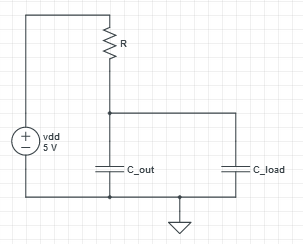
\includegraphics [scale = 0.5] {figures/PDN_schematic}
 \caption{Vereenvoudigde schakeling van het PDN, op \emph{t = 0} is de spanning over \emph{C\tss{load}} gelijk aan \emph{5V}}
 \label{res:PDN_schematic}
 \end{center}
 \end{figure}

 \begin{figure} [h!]
 \begin{center}
 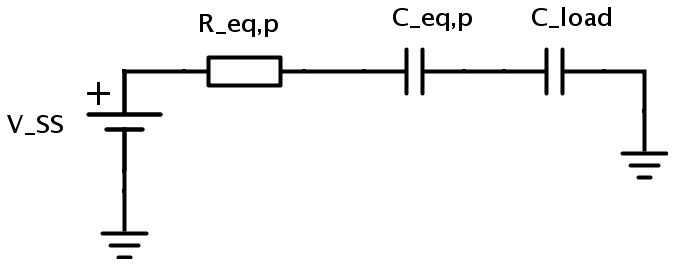
\includegraphics [scale = 0.5] {figures/PUN_schematic}
 \caption{Vereenvoudigde schakeling van het PUN, op \emph{t = 0} is de spanning over \emph{C\tss{load}} gelijk aan \emph{0V}}
 \label{res:PUN_schematic}
 \end{center}
 \end{figure}

\begin{enumerate}

%%%STAP 1%%%
\item \textbf{Stroom bepalen door de transistor d.m.v. SPICE model}\\
Als eerst moet de stroom worden bepaald door de transistor, dit moet tweemaal gedaan worden voor zowel het PDN als het PUN gedeelte. Voor het bepalen van de capaciteit van het PDN moeten de twee inputs van de NAND worden aangesloten op \emph{V\tss{SS}} en zal de spanning over de variabele belastingscapaciteit \emph{C\tss{load}} op \emph{t = 0} gelijk zijn aan \emph{5V}. Op deze manier staat het PUN dicht en het PDN open en kan de stroom gemeten worden door het PDN. Voor het bepalen van de capaciteit van het PUN moeten de twee inputs van de NAND worden aangesloten op de ground. Op deze manier kan de stroom worden bepaald door het PUN.

%%%STAP 2%%%
\item \textbf{Stroom bepalen op \emph{t = 0}}\\
Om \emph{R\tss{eq,n}} te bepalen moet de stroom door de transistor worden bepaald op \emph{t = 0}. Op dit tijdstip zal, wanneer \emph{V\tss{in} = V\tss{SS}} en de spanning over \emph{C\tss{load}} gelijk is aan \emph{5V}, het PUN dicht zijn en het PDN open zijn.  De capaciteiten \emph{C\tss{load}} en \emph{C\tss{out,n}} zijn op dat tijdstip opgeladen en zullen zich langzaam ontladen. De \emph{R\tss{eq,n}} kan dan worden bepaald aan de hand van de volgende formule:

\begin{equation}
R\tss{eq,n} = \frac{5V}{i\tss{n}(0)}
\end{equation}

Om \emph{R\tss{eq,p}} te bepalen moet ook de stroom worden bepaald op \emph{t = 0}. Ditmaal is \emph{V\tss{in} = 0V} en de spanning over \emph{C\tss{load}} gelijk aan \emph{V\tss{SS}}. De capaciteiten \emph{C\tss{load}} en \emph{C\tss{out,p}} zijn op dit tijdstip ontladen en zullen zich langzaam opladen. De \emph{R\tss{eq,p}} kan dan worden bepaald aan de hand van de volgende formule:

\begin{equation}
R\tss{eq,p} = \frac{V\tss{SS}}{i\tss{p}(0)}
\end{equation}

%%%STAP 3%%%
\item \textbf{De RC tijd bepalen}\\
Om de RC tijd voor het PDN $\tau$\tss{n} uit figuur \ref{res:PDN_schematic} te bepalen en de RC tijd voor het PUN $\tau$\tss{p} uit figuur \ref{res:PUN_schematic} te bepalen moeten we eerst voor beide schakelingen een functie voor de stroom bepalen. Dit kan aan de hand van de volgende formule uit het Lineaire Schakelingen boek [2], p. 307:

\begin{equation}
i(t) = i(\infty) + [i(0+) - i(\infty)]e\tsss{-t/$\tau$}
\end{equation}

Als we deze formule invullen krijgen we:

\begin{equation}
i\tss{n}(t) = \frac{5V}{R\tss{eq,n}}e\tsss{-t/$\tau$} = i(0)\tss{n}e\tsss{-t/$\tau$\tss{n}}
\end{equation}

\begin{equation}
i\tss{p}(t) = \frac{V\tss{SS}}{R\tss{eq,p}}e\tsss{-t/$\tau$} = i(0)\tss{p}e\tsss{-t/$\tau$\tss{p}}
\end{equation}

Als we deze formules omschrijven krijgen we voor het PDN:

\begin{equation}
\tau\tss{n} = \frac{-t}{ln(\frac{i\tss{n}(t)}{i\tss{n}(0)})}
\end{equation}

En voor het PUN krijgen we:

\begin{equation}
\tau\tss{p} = \frac{-t}{ln(\frac{i\tss{p}(t)}{i\tss{p}(0)})}
\end{equation}

Hierbij kan de waarde \emph{t} en de waarde \emph{i(t)} uit de stroom karakteristiek worden afgelezen die is opgesteld bij stap 1.

%%%STAP 4%%%
\item \textbf{\emph{C\tss{out,n}} en \emph{C\tss{out,p}} berekenen aan de hand van $\tau$}\\
Als laatst kunnen de \emph{C\tss{out,n}} en \emph{C\tss{out,p}} berekend worden d.m.v. de RC tijd:

\begin{equation}
\tau = R\tss{eq}C\tss{eq} = R\tss{eq}(\frac{C\tss{out}C\tss{load}}{C\tss{eq} + C\tss{load}})
\end{equation}

Als we deze formule omschrijven krijgen we een functie die de \emph{C\tss{out,n}} en \emph{C\tss{out,p}} kan bepalen:

\begin{equation}
C\tss{eq,n} = \frac{\frac{\tau\tss{n}}{R\tss{eq,n}}C\tss{load}}{C\tss{load} - \frac{\tau\tss{n}}{R\tss{eq,n}}}
\end{equation}

\begin{equation}
C\tss{eq,p} = \frac{\frac{\tau\tss{p}}{R\tss{eq,p}}C\tss{load}}{C\tss{load} - \frac{\tau\tss{p}}{R\tss{eq,p}}}
\end{equation}


\end{enumerate}

\end{document}